% Customizable fields and text areas start with % >> below.
% Lines starting with the comment character (%) are normally removed before release outside the collaboration, but not those comments ending lines

% svn info. These are modified by svn at checkout time.
% The last version of these macros found before the maketitle will be the one on the front page,
% so only the main file is tracked.
\RCS$Revision$
\RCS$HeadURL$
\RCS$Id$

%%%%%%%%%%%%% local definitions %%%%%%%%%%%%%%%%%%%%%
% This allows for switching between one column and two column (cms@external) layouts
% The widths should  be modified for your particular figures. You'll need additional copies if you have more than one standard figure size.
\newlength\cmsFigWidth
\ifthenelse{\boolean{cms@external}}{\setlength\cmsFigWidth{0.85\columnwidth}}{\setlength\cmsFigWidth{0.4\textwidth}}
\ifthenelse{\boolean{cms@external}}{\providecommand{\cmsLeft}{top\xspace}}{\providecommand{\cmsLeft}{left\xspace}}
\ifthenelse{\boolean{cms@external}}{\providecommand{\cmsRight}{bottom\xspace}}{\providecommand{\cmsRight}{right\xspace}}
\setcounter{tocdepth}{3}

\def\IP{\ensuremath{\hat{\mathrm{IP}}^\mathrm{2D}_\mathrm{sig}}\xspace}
\def\TA{\ensuremath{\hat{\Theta}^\mathrm{2D}}\xspace}
\def\AL{\ensuremath{\alpha_\mathrm{max}}\xspace}
\def\NT{\ensuremath{N_{\mathrm{displaced-tag}}}\xspace}
\def\ptossf{\pt($\ell^+\ell^-$)\xspace}
\def\dilepton{\ensuremath{\ell^+\ell^-}\xspace}
\def\emu{\ensuremath{\ell^+\ell'^-}\xspace}
\def\Z{\ensuremath{\mathrm{Z}}\xspace}
\def\ZL{\ensuremath{\mathrm{Z}_{\mathrm{low-p_{T}}}}\xspace}
\def\ZH{\ensuremath{\mathrm{ZH}}\xspace}
\def\heavy{\ensuremath{\mathrm{t\bar{t}}+\mathrm{top}}\xspace}
\def\WW{\ensuremath{\mathrm{W^{+}W^{-}}}\xspace}
\def\ZZ{\ensuremath{\mathrm{ZZ}}\xspace}
\def\WZ{\ensuremath{\mathrm{W^{\pm}Z}}\xspace}
\def\DY{\ensuremath{\mathrm{Z}/\gamma^{*}}\xspace}
%\def\twoeledy{\ensuremath{\mathrm{TwoEleLowPt}}\xspace}
\def\twoeledy{\ensuremath{\mathrm{Z(}e^+e^-\mathrm{)}_\mathrm{low-p_{T}}}\xspace}
%\def\twomudy{\ensuremath{\mathrm{TwoMuLowPt}}\xspace}
\def\twomudy{\ensuremath{\mathrm{Z(}\mu^+\mu^-\mathrm{)}_\mathrm{low-p_{T}}}\xspace}
%\def\twomuzh{\ensuremath{\mathrm{TwoMuHighPt}}\xspace}
\def\twoelezh{\ensuremath{\mathrm{Z(}e^+e^-\mathrm{)}_\mathrm{high-p_{T}}}\xspace}
\def\twollzh{\ensuremath{\mathrm{Z(}\ell^+\ell^-\mathrm{)}_\mathrm{high-p_{T}}}\xspace}
\def\twolldy{\ensuremath{\mathrm{Z(}\ell^+\ell^-\mathrm{)}_\mathrm{low-p_{T}}}\xspace}
%\def\twoelezh{\ensuremath{\mathrm{Z}_{e^+e^-}^\mathrm{high-p_{T}}}\xspace}
%\def\twoelezh{\ensuremath{\mathrm{TwoEleHighPt}}\xspace}
\def\twomuzh{\ensuremath{\mathrm{Z(}\mu^+\mu^-\mathrm{)}_\mathrm{high-p_{T}}}\xspace}
\def\elemulow{\ensuremath{\mathrm{EleMuLowPt}}\xspace}
\def\elemul{\ensuremath{\mathrm{Top(}e\mu\mathrm{)}_\mathrm{low-p_{T}}}\xspace}
\def\elemu{\ensuremath{\mathrm{Top(}e\mu\mathrm{)}_\mathrm{high-p_{T}}}\xspace}
\def\elemuall{\ensuremath{\mathrm{Top(}e\mu\mathrm{)}}\xspace}
\def\NTAGS{\ensuremath{\mathrm{N}_{j}^{\mathrm{dis}}}\xspace}
%\usepackage{cleveref}
%%%%%%%%%%%%%%%  Title page %%%%%%%%%%%%%%%%%%%%%%%%

\cmsNoteHeader{AN-00-000} % This is over-written in the CMS environment: useful as preprint no. for export versions
% >> Title: please make sure that the non-TeX equivalent is in PDFTitle below
\title{Search for Higgs boson decays to long-lived scalar particles to $\tau$ final state with Regions of Interest}

% >> Authors
%Author is always "The CMS Collaboration" for PAS and papers, so author, etc, below will be ignored in those cases
%For multiple affiliations, create an address entry for the combination
%To mark authors as primary, use the \author* form
\address[Rutgers]{Rutgers, The State University of New Jersey}
\address[DESY]{Deutsches Elektronen-Synchrotron}
\address[fsu]{Florida State University}
\author[DESY]{L. Benato}
\author[Rutgers]{Y. Gerstein}
\author[Rutgers]{A. Hart}
\author[fsu]{S. Kim}
\author[fsu]{T. Kolberg}
\author[DESY]{K. Pe\~na}
\author[Rutgers]{K. Rahman}
% >> Date
% The date is in yyyy/mm/dd format. Today has been
% redefined to match, but if the date needs to be fixed, please write it in this fashion.
% For papers and PAS, \today is taken as the date the head file (this one) was last modified according to svn: see the RCS Id string above.
% For the final version it is best to "touch" the head file to make sure it has the latest date.
\date{\today}

% >> Abstract
% Abstract processing:
% 1. **DO NOT use \include or \input** to include the abstract: our abstract extractor will not search through other files than this one.
% 2. **DO NOT use %**                  to comment out sections of the abstract: the extractor will still grab those lines (and they won't be comments any longer!).
% 3. For PASs: **DO NOT use tex macros**         in the abstract: CDS MathJax processor used on the abstract doesn't understand them _and_ will only look within $$. The abstracts for papers are hand formatted so macros are okay.
\abstract{
   We present a search for long-lived particles (LLPs) produced in gluon fusion Higgs production mode (ggH), using the novel Regions of Interest strategy. Regions of Interest (ROIs) are formed as a collection of pair-wise track vertices fitted by the V0Fitter in CMSSW.
   The analysis focuses on lifetime of LLPs in the tracker region, with concentration on the ggH mode for the highest Higgs production cross-section.
   Variables of the constructed ROIs become inputs for our Deep Neural Network (DNN) Machine Learning (ML) algorithms, as a main distriminator between the signal and the background. 
   We focus on the SM $\tau$ final state. This final state is particulary interesting, given $\tau$ final state exclusion limits are frequently omitted in precedent analysis, due to $\tau$ leptons' non trivial reconstruction mechanism.
  No excess of events over the standard model expectation is observed.
  The results are interpreted in the context of exotic Higgs decays to a pair of long-lived scalars ($S$).
  We set limits on the branching ratio of the Higgs to LLPs, \textbf{B}(H$\rightarrow SS$)
  , as a function of the proper lifetime. 
 % The expected limits
 % constrain the \textbf{B}(H$\rightarrow SS$) to be below $\sim$4-5~\% ($\sim$15\%) for masses
 % of 40-55~\GeV (15~\GeV) and proper lifetimes of 10-100~\mm (10-50~\mm).
}

% >> PDF Metadata
% Do not comment out the following hypersetup lines (metadata). They will disappear in NODRAFT mode and are needed by CDS.
% Also: make sure that the values of the metadata items are sensible and are in plain text:
% (1) no TeX! -- for \sqrt{s} use sqrt(s) -- this will show with extra quote marks in the draft version but is okay).
% (2) no %.
% (3) No curly braces {}.
\hypersetup{%
pdfauthor={S. Kim},%
pdftitle={Search for Higgs boson decays to long-lived scalar particles to $\tau$ final state with Regions of Interest},%
pdfsubject={CMS},%
pdfkeywords={CMS, physics}}

\maketitle %maketitle comes after all the front information has been supplied
% >> Text
%%%%%%%%%%%%%%%%%%%%%%%%%%%%%%%%  Begin text %%%%%%%%%%%%%%%%%%%%%%%%%%%%%
%% **DO NOT REMOVE THE BIBLIOGRAPHY** which is located before the appendix.
%% You can take the text between here and the bibiliography as an example which you should replace with the actual text of your document.
%% If you include other TeX files, be sure to use "\input{filename}" rather than "\input filename".
%% The latter works for you, but our parser looks for the braces and will break when uploading the document.
%%%%%%%%%%%%%%%
\tableofcontents
\clearpage

\section{Introduction}\label{sec:introduction}

Discovery of particles at the electroweak scale, such as the top quark at Fermilab's CDF and D0~\cite{topD0,topCDF} and the Higgs Boson at Large Hadron Collider (LHC) in CERN~\cite{higgscms,higgsatlas}, led to discovery of all constituents in the standard model (SM). 
SM helps to describe the nature of fundamental particles and their interactions with precision. 
In spite of its success, the SM suffers from a few obstacles. 
The evidence of neutrino mass and mixing~\cite{neutrino}, the observation of bullet clusters confirming the presence of dark matter (DM)~\cite{Baumgart:2009tn,Kaplan:2009ag,Chan:2011aa,Dienes:2011ja,Dienes:2012yz}, and baryon-antibaryon asymmetry~\cite{Cui:2014twa} remain unsolved in framework of the SM. 
In addition, SM suffers from the naturalness problem. 
To solve all such issues, one needs to look for Beyond the Standard Model (BSM).

The naturalness problem originates from the fact that the Higgs of the SM is a scalar particle. 
Unlike fermions or gauge bosons, its mass is not protected by any symmetry and subject to large radiative corrections, especially from the top quark loop. 
Thus, for the SM to be valid up to the Planck or Grand Unification Theory (GUT) scale, the radiative corrections are enormous. 
One needs un-natural amount of fine tuning to fit the Higgs mass at the observed value of 125GeV.
One of the most popular solutions to this problem is Supersymmetry (SUSY), which assigns chirality to the Higgs particle. 
SUSY solves correction problem, neutrino masses, and provides candidate of DM. 
Unfortunately, LHC has found no significant excess over the SM background in their search for SUSY\cite{SUSY}. 
Although the non-observation of superpartners does not invalidate SUSY, it makes less attractive among the particle physics community. 
Non-observation of superpartners, particularly the stop (scalar partner of the top quark) has pushed its mass beyond 1TeV. 
This generated problem of "little hierarchy", but an alternative solution of "neutral naturalness" remains. 

In the framework of neutral naturalness, top partners are not charged under the SM color group. 
Because of being colorless, its cross-section of production is much less, and the present limits on the top partner particles are well below 1TeV. 
Examples of neutral naturalness models are Twin Higgs \cite{Chacko:2005pe},
Folded SUSY \cite{Burdman:2006tz}, and Quirky Little Higgs \cite{Cai:2008au}.
Theoretical models provide the possibility of neutral Long Lived Particles (LLPs), which may be produced in the proton-proton
collisions of the LHC and decay back to SM particles far from the interaction point (IP).\cite{Craig:2015pha}
In the Mirror and Twin SM models, only SM Higgs boson can interact with both SM QCD and mirror QCD partners.
If the mirror QCD gluons could form scalar glueballs, the SM Higgs boson can become "Higgs Portal" between the SM and BSM mirror QCD scalar glueballs. 
BSM mirror QCD scalar glueballs can only decay back to SM particles via Higgs portal as well. 
Because of its decay as an offshell Higgs boson, its crosssection is highly suppressed. 
Decay branching ratio to highest mass fermions will be highest following the Yukawa couplings.
Decay ratio into b quarks or tau leptons are highest depending on the mirror scalar's mass.
The displaced decays of the scalars will lead to exotic signatures in the LHC, such as distant innermost tracker hit, displaced vertices, and displaced jets.
Phenomenology of long-lived particles in LHC entailed increase in interest of neutral naturalness framework among the particle physics community. \cite{Curtin:2015fna,Csaki:2015fba}.
The long-lived scalar model is shown in the left-panel of Figure~\ref{fig:twinhiggs}.


Searches for LLPs decaying into final states containing jets were investigated
at the Tevatron ( $\sqrt{s}$ = 1.96~TeV) by both CDF~\cite{Aaltonen:2011rja} and D0~\cite{Abazov:2009ik} Collaborations,
at the LHC by the ATLAS and LHCb Collaborations at $\sqrt{s}$ = 7~TeV~\cite{ATLAS:2012av,Aaij:2014nma},
by the ATLAS,CMS and LHCb Collaborations at $\sqrt{s}$ = 8~TeV~\cite{Aad:2015uaa,Aad:2015rba,PhysRevD.91.012007,Aad:2015asa,Aaij:2017mic,Aaij:2016xmb,Aaij:2015ica}.
More recently, CMS Collaboration~\cite{Sirunyan:2017jdo,displacedvertices,displacedjets2016,delayedjets,emergingjets,CMS-PAS-EXO-19-021}
 and ATLAS Collaboration~\cite{Aaboud:2018iil,Aaboud:2018jbr,Aaboud:2018arf,Aaboud:2018aqj,Aaboud:2018kbe,Aaboud:2019trc,Aaboud:2019opc,Aad:2019kiz,Aad:2019pfm,Aad:2019tcc,Aad:2019xav,Aad:2019tua} at $\sqrt{s}$ = 13~TeV. 
CMS Collaboration released a new result in 2021, in which Higgs are created in association with Z vector boson ~\cite{ZHAN}, for better probe into lighter scalar mass thanks to its clean dilepton trigger.

Although exclusion limit on b and d-quarks were set below 1 for analyses above, exclusion limit for $\tau$ final state has been frequently omitted or presented with values above 1.  
Displaced Jets analyses face challenges for $\tau$ final state, due to $\tau$'s non-trivial hadronic and leptonic decay mode and complicated reconstruction mechanism. 
However, Leptophilic model for Twin Higgs and other Higgs models are also highly motivated ~\cite{Lepto}. Continuous neglect of $\tau$ final state limit is not only a good practice, but overlooking an important undiscovered phase space. 
This analysis searches for Higgs Portal model with the Higgs' Leptophilic nature, which focuses on $\tau$ final state.
The 55GeV maximum mass is to investigate only on-shell neutral scalar particles from the Higgs. 
Minimum 7GeV of scalar particles' mass is required to create on-shell tau-lepton pairs.
Feynman diagram of the scalar particle production mechanism is depicted in figure 1.

Most CMS searches are not optimal for detecting Higgs boson decays to displaced-jets
due to the soft $p_T$ nature of its decays products -- the new scalars.
%Standard CMS searches rely on $H_T$ triggers that are highly inefficienty for this signal.
Low HT signature becomes particularly more difficult with long lived signature.
Higgs produced in association with Z vector boson analysis~\cite{ZHAN} overcame this barrier with help of dilepton trigger. 
Although ggH production mode gives the largest Higgs crosssection, it complicates the trigger strategy even further. 
This analysis exploits the $\tau$ lepton's leptonic decay mode, in which the $\tau$ lepton decays into a soft muon, with trigger of B Parking HLT Path implemented in CMS for the year 2018 of Run2.

Another challenge for $\tau$ lepton analysis is different decay modes of $\tau$ leptons. 
$\tau$ leptons decay hadronically and leptonically with several different sub-decay modes. 
Developing analysis strategies to optimize search for each sub-decay modes are extremely complicated, a main reason for omission or no good exclusion limit in precedent LHC results.
To be inclusive of all $\tau$ leptons' decay modes, displaced vertex serach can be more efficient than displace object (jet,muon,electrons). 
We exploit the newly developed Regions of Interest mechanism in the tracker volume. 
Regions of Interest (ROI) form displaced vertex candidates, by fittng pair-wise tracks of Lost-tracks and PackedPFCandidates classes in MINIAOD into a vertex. 
ROIs save all relevant track and fitted vertex qualities along with isolation informaiton.
These variables are used as input for Machine Learning (ML) algorithms, enabling a highly generic and data-scientific search method.


The rest of this note is organized as follows.
In Section~\ref{sec:samples}, we describe the datasets and Monte Carlo samples, including those of the signal model, used in the search. 
The physics objects and formation of Regions of Interest are described in Section~\ref{sec:objects}.
The trigger strategy and event selections are presented in Section~\ref{sec:selections}. 
Section~\ref{sec:estimate} describes the data driven background estimate and its validation. 
Section~\ref{sec:systs} describes the systematic uncertainties.
Finally, Section~\ref{sec:results} presents the results of the search.
We conclude with Section~\ref{sec:conclusions}.

\clearpage

\section{Data and simulated samples}\label{sec:samples}

\subsection{Data samples}

The analysis uses B Parking datasets. Data was
collected during 2018 of Run 2and corresponds to an integrated luminosity of
 41~$\mathrm{fb}^{-1}$.

\begin{table}[htb!]
  \caption{Datasets used in the analysis:and 2018.}
  \begin{center}
    %\footnotesize
    %\scriptsize
    \begin{tabular}{l|l}\hline
      Data sample & Integrated Luminosity (fb$^-1$)\\
      \hline
      /ParkingBPH1/Run2018A-05May2019-v1/MINIAOD  & 0.866 \\
      /ParkingBPH2/Run2018A-05May2019-v1/MINIAOD  & 0.866 \\
      /ParkingBPH3/Run2018A-05May2019-v1/MINIAOD  & 0.866 \\
      /ParkingBPH4/Run2018A-05May2019-v1/MINIAOD  & 0.866 \\
      /ParkingBPH5/Run2018A-05May2019-v1/MINIAOD  & 0.866 \\
      /ParkingBPH6/Run2018A-05May2019-v1/MINIAOD  & 0.866 \\
      Total & 5.20\\
      \hline
      /ParkingBPH1/Run2018B-05May2019-v2/MINIAOD  & 1.083 \\
      /ParkingBPH2/Run2018B-05May2019-v2/MINIAOD  & 1.083 \\
      /ParkingBPH3/Run2018B-05May2019-v2/MINIAOD  & 1.083 \\
      /ParkingBPH4/Run2018B-05May2019-v2/MINIAOD  & 1.083 \\
      /ParkingBPH5/Run2018B-05May2019-v2/MINIAOD  & 1.083 \\
      /ParkingBPH6/Run2018B-05May2019-v2/MINIAOD  & 1.083 \\
      Total & 6.49\\
      \hline
      /ParkingBPH1/Run2018C-05May2019-v1/MINIAOD  & 1.079 \\
      /ParkingBPH2/Run2018C-05May2019-v1/MINIAOD  & 1.079 \\
      /ParkingBPH3/Run2018C-05May2019-v1/MINIAOD  & 1.079 \\
      /ParkingBPH4/Run2018C-05May2019-v1/MINIAOD  & 1.079 \\
      /ParkingBPH5/Run2018C-05May2019-v1/MINIAOD  & 1.079 \\
      Total & 5.39\\
      \hline
      /ParkingBPH1/Run2018D-05May2019promptD-v1/MINIAOD  & 6.542 \\
      /ParkingBPH2/Run2018D-05May2019promptD-v1/MINIAOD  & 6.542 \\
      /ParkingBPH3/Run2018D-05May2019promptD-v1/MINIAOD  & 6.542 \\
      /ParkingBPH4/Run2018D-05May2019promptD-v1/MINIAOD  & 6.542 \\
      /ParkingBPH5/Run2018D-05May2019promptD-v1/MINIAOD  & 6.542 \\
      Total & 32.7\\
      \hline
      ParkingBPH Total & 50.78 \\
      \hline
    \end{tabular}
    \label{tab:datasample2018BPH}
  \end{center}
\end{table}


%We process the data included in the Cert\_271036-284044\_13TeV\_23Sep2016ReReco\_Collisions16\_JSON.txt JSON file.


\subsection{Monte Carlo Samples}

\subsubsection{Signal Model and Simulation}

The ggH process (see Figure~\ref{fig:feynmanggH}) is generated at next-to-next-to-leading order (NNLO) and next-to-next-to-leading-log (NNLL) QCD and next-to-leading order (NLO) EW accuracies ~\cite{Heinemeyer:2013xd}.
The Higgs boson mass is set to 125~\GeV for all signal samples.
The cross sections, computed at NNLO+NNLL QCD and NLO EW accuracies and obtained from the
CERN Report 3,
are 4.414~$\mathrm{pb}$. The CMS detector response is modeled with GEANT4~\cite{Agostinelli:2002hh}.

\begin{figure}[h!]
  \caption{Leading Feynman diagrams for ggH production mode}
  \label{fig:feynmanggH}
  \centering
  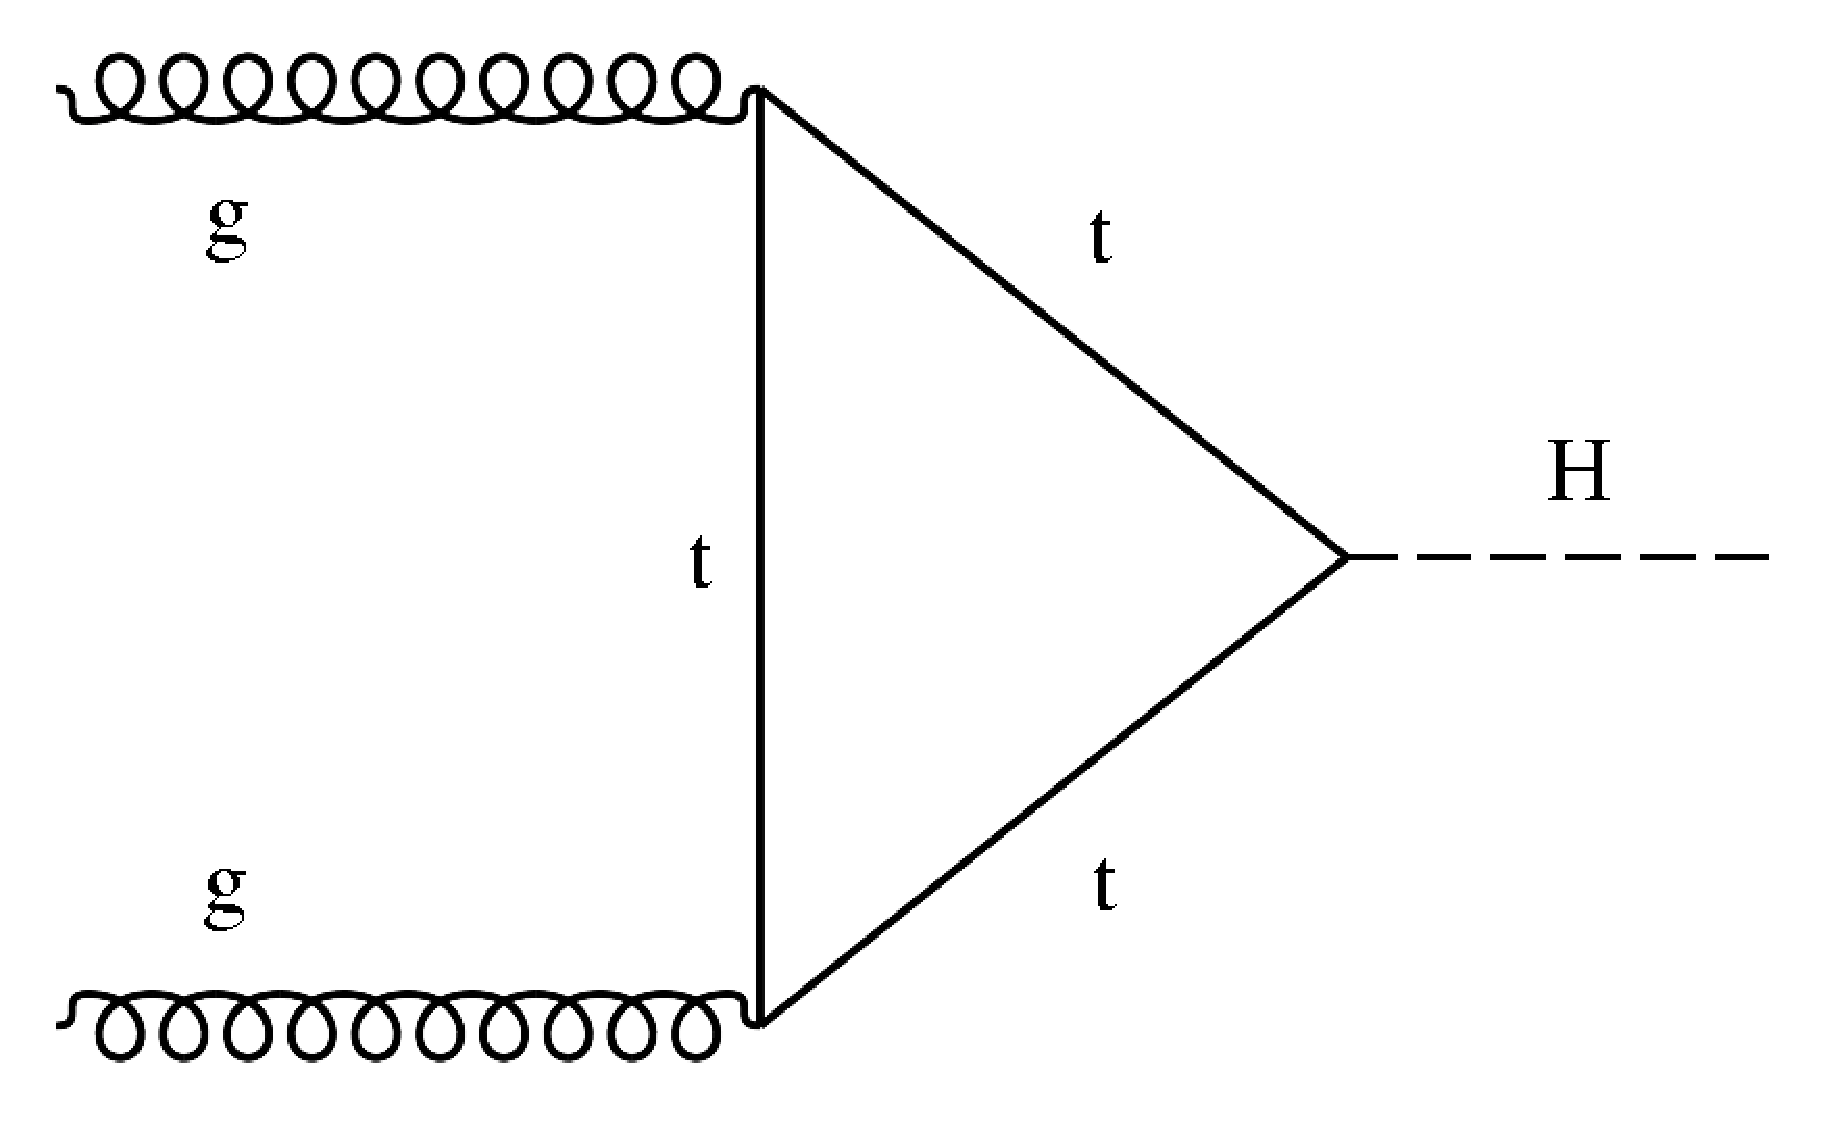
\includegraphics[width=0.47\linewidth]{figs/feynmanggH.pdf}

\end{figure}


%The Higgs boson decay to long-lived scalars is simulted using \PYTHIA v8.230~\cite{Sjostrand:2014zea}.
%The parton distribution functions used to produce all samples are the
%next-to-next-to-leading order (NNLO) NNPDF3.1 set~\cite{Ball:2017nwa}.
%For parton showering and hadronization, the matrix element generators are interfaced
%with \PYTHIA v8.230. For all samples, simulated additional pp interactions (pileup)
% are added to the hard-scattering process with the multiplicity distribution matched
% to the corresponding data-taking period (2016, 2017, 2018).
%The scalar is simulated as a generic scalar particle with a 100\% branching
%ratio to b-quarks (samples with scalar decays to light quarks and tau
%leptons also exist).
%We generate samples with varying scalar mass and lifetime, and include in this
%set of variations the
%benchmark points recommended by the LHCHXSWG~\cite{deFlorian:2016spz}.
Table~\ref{tab:sigsample} lists the signal Monte Carlo samples.

%%%%%%%%% %%%%%%%%%%%%%%%%%%%%%%%%%%%%%%%%%%%%%%%%%%%%%%%%%%%%%%%%%%%%%%%%%%%%%%%%
% The tables below are generated from lines like `python check_used.py | grep HToBB`
% using the script in LLDJstandalones/lists/ntuple
%%%%%%%%%%%%%%%%%%%%%%%%%%%%%%%%%%%%%%%%%%%%%%%%%%%%%%%%%%%%%%%%%%%%%%%%%%%%%%%%%%%%%%%%

\begin{table}[htb]
  % campaign: $\mathrm{RunIISummer16DR80Premix\-PUMoriond17\_80X\_mcRun2\_asymptotic\_2016\_TrancheIV\_v6\-v1}$.}
  \caption{gg($h \rightarrow ss\rightarrow \tau\bar{\tau} \tau\bar{\tau}$) Signal Monte Carlo samples.}
  \begin{center}
    %\footnotesize
    \scriptsize
    \begin{tabular}{l}\hline
      Sample \\
      \hline
      /ggH\_HToSSTo4Tau\_MH-125\_TuneCP5\_13TeV-powheg-pythia8/CAMPAIGN/MINIAODSIM\\
      \hline
      /ggH\_HToSSTo4Tau\_MH-125\_MS-55\_ctauS-1\_TuneCP5\_13TeV-powheg-pythia8/CAMPAIGN/MINIAODSIM\\
      /ggH\_HToSSTo4Tau\_MH-125\_MS-55\_ctauS-10\_TuneCP5\_13TeV-powheg-pythia8/CAMPAIGN/MINIAODSIM\\
      /ggH\_HToSSTo4Tau\_MH-125\_MS-55\_ctauS-100\_TuneCP5\_13TeV-powheg-pythia8/CAMPAIGN/MINIAODSIM\\
      /ggH\_HToSSTo4Tau\_MH-125\_MS-55\_ctauS-1000\_TuneCP5\_13TeV-powheg-pythia8/CAMPAIGN/MINIAODSIM\\
      /ggH\_HToSSTo4Tau\_MH-125\_MS-40\_ctauS-1\_TuneCP5\_13TeV-powheg-pythia8/CAMPAIGN/MINIAODSIM\\
      /ggH\_HToSSTo4Tau\_MH-125\_MS-40\_ctauS-10\_TuneCP5\_13TeV-powheg-pythia8/CAMPAIGN/MINIAODSIM\\
      /ggH\_HToSSTo4Tau\_MH-125\_MS-40\_ctauS-100\_TuneCP5\_13TeV-powheg-pythia8/CAMPAIGN/MINIAODSIM\\
      /ggH\_HToSSTo4Tau\_MH-125\_MS-40\_ctauS-1000\_TuneCP5\_13TeV-powheg-pythia8/CAMPAIGN/MINIAODSIM\\
      /ggH\_HToSSTo4Tau\_MH-125\_MS-15\_ctauS-1\_TuneCP5\_13TeV-powheg-pythia8/CAMPAIGN/MINIAODSIM\\
      /ggH\_HToSSTo4Tau\_MH-125\_MS-15\_ctauS-10\_TuneCP5\_13TeV-powheg-pythia8/CAMPAIGN/MINIAODSIM\\
      /ggH\_HToSSTo4Tau\_MH-125\_MS-15\_ctauS-100\_TuneCP5\_13TeV-powheg-pythia8/CAMPAIGN/MINIAODSIM\\
      /ggH\_HToSSTo4Tau\_MH-125\_MS-15\_ctauS-1000\_TuneCP5\_13TeV-powheg-pythia8/CAMPAIGN/MINIAODSIM\\
      /ggH\_HToSSTo4Tau\_MH-125\_MS-7\_ctauS-1\_TuneCP5\_13TeV-powheg-pythia8/CAMPAIGN/MINIAODSIM\\
      /ggH\_HToSSTo4Tau\_MH-125\_MS-7\_ctauS-10\_TuneCP5\_13TeV-powheg-pythia8/CAMPAIGN/MINIAODSIM\\
      /ggH\_HToSSTo4Tau\_MH-125\_MS-7\_ctauS-100\_TuneCP5\_13TeV-powheg-pythia8/CAMPAIGN/MINIAODSIM\\
      /ggH\_HToSSTo4Tau\_MH-125\_MS-7\_ctauS-1000\_TuneCP5\_13TeV-powheg-pythia8/CAMPAIGN/MINIAODSIM\\
      \hline
    \end{tabular}
    \label{tab:sigsample}
  \end{center}
\end{table}




An example \PYTHIA v8.230 fragment for the Higgs decay to scalars (scalars) and their subsequent decay to tau leptons is given below.
In this example the mass of the scalar is 15~\GeV and its lifetime ($\mathrm{c}\tau$) is 10,000~\mm.
\begin{verbatim}
  '9000006:all = sk skbar 0 0 0 15 1.9732e-17 1.0 75.0 10000',
  '9000006:oneChannel = 1  1.0 101  15 -15',
  '9000006:mayDecay = on',
  '9000006:isResonance = on',
  '25:m0 = 125.0',
  '25:onMode = off',
  '25:addChannel = 1 0.000000001 101 9000006 -9000006',
  '25:onIfMatch = 9000006 -9000006',
  '9000006:onMode = off',
  '9000006:onIfAny = 5',
\end{verbatim}


%Figure~\ref{fig:scalarpt} (left) and Figure~\ref{fig:zd_scalarpt} (left)
%show the Monte Carlo truth level distributions for the scalar ($S$) and $Z_{d}$ \pt, respectively.
%These distributions exhibit the soft-\pt nature of signal models.
%Figure~\ref{fig:scalarpt} (right) nd Figure~\ref{fig:zd_scalarpt} (right) show
% the Monte Carlo truth level distributions of the
%$\Delta R$ between the decay products of the scalar ($S$) and $Z_{d}$ for different masses.
%Note that significant portions of the distributions lie within the common jet radius of 0.4.
%Both of these figures show a signal with scalar decays to tau leptons to kinematically allow
%a lower scalar mass of 7~\GeV.
%
%\begin{figure}[h!]
%  \caption{\pt of the scalar ($s$) decay products (left) and
%  $\Delta R$ between the two scalar decay products (right) for different masses.
%  For the scalar masses below the $\mathrm{b}\mathrm{\bar{b}}$ threshold
%  the scalar decays into $\mathrm{d}\mathrm{\bar{d}}$.}
%  \label{fig:scalarpt}
%  \centering
%  %\includegraphics[width=0.47\linewidth]{figs/scalarpt.pdf}
%  %\includegraphics[width=0.45\linewidth]{figs/dr_lead_tautau.pdf}
%  \includegraphics[width=0.47\linewidth]{figs/dScalar_pT100mm.pdf}
%  \includegraphics[width=0.45\linewidth]{figs/dScalar_dR100mm.pdf}
%  %\SK placeholder\includegraphics[width=0.47\linewidth]{figs/Zdark_pT.pdf}
%  %\SK placeholder\includegraphics[width=0.45\linewidth]{figs/Zdark_dR.pdf}
%\end{figure}
%
%
%\begin{figure}[h!]
%  \caption{\pt of the $Z_{d}$ decay products (left)
%  and $\Delta R$ between the two $Z_{d}$ decay products (right) for different masses.}
%  \label{fig:zd_scalarpt}
%  \centering
%  \includegraphics[width=0.47\linewidth]{figs/Zdark_pT.pdf}
%  \includegraphics[width=0.47\linewidth]{figs/Zdark_dR.pdf}
%\end{figure}
%
%
%Figure~\ref{fig:flightdist} and Figure~\ref{fig:zd_flightdist} show the flight distances in the lab-frame
%for different scalar ($S$) and $Z_{d}$ proper-lifetimes, respectively.
%Figure~\ref{fig:Zdark_pT} shows the Z boson \pt distribution for different
%heavy scalar ($\Phi$) and $Z_{d}$ masses. The Z boson \pt starts to be well above
%the 100~\GeV threshold set by the background estimation method (see Section~\ref{sec:searhregion})
%for $\Phi$ masses ($m_{\Phi}$) above 250~\GeV. Therefore, we focus the model interpretation
%in the scenarios where $m_{\Phi} > 250$~\GeV.
%
%\begin{figure}[h!]
%  \caption{LLP flight distance in lab-frame for different scalar lifetimes and masses.
%  For the scalar masses below the $\mathrm{b}\mathrm{\bar{b}}$ threshold
%  the scalar decays into $\mathrm{d}\mathrm{\bar{d}}$.
%  }
%  \label{fig:flightdist}
%  \centering
%  \includegraphics[width=0.47\linewidth]{figs/dScalar_dist_7GeV.pdf}
%  \includegraphics[width=0.47\linewidth]{figs/Scalar_MS15.pdf}
%  \includegraphics[width=0.47\linewidth]{figs/Scalar_MS40.pdf}
%  \includegraphics[width=0.47\linewidth]{figs/Scalar_MS55.pdf}
%\end{figure}
%
%\begin{figure}[h!]
%  \caption{LLP flight distance in lab-frame for different $Z_{d}$ lifetimes and masses.
%   Information is MC-thruth
%  }
%  \label{fig:zd_flightdist}
%  \centering
%  \includegraphics[width=0.47\linewidth]{figs/Zd_ctau_llp20.pdf}
%  \includegraphics[width=0.47\linewidth]{figs/Zd_ctau_llp50.pdf}
%\end{figure}
%
%\begin{figure}[h!]
%  \caption{$Z$ $p_{T}$ comparison for a scalar mass ($\Phi$) of 50~\GeV.
%   $Z_{d}$ mass of  20~\GeV (left)  and 50~\GeV (right).
%  }
%  \label{fig:Zdark_pT}
%  \centering
%  \includegraphics[width=0.47\linewidth]{figs/Zdark_Zpt175llp20.pdf}
%  \includegraphics[width=0.47\linewidth]{figs/Zdark_Zpt175llp50.pdf}
%\end{figure}

\subsubsection{Background Monte Carlo}
All samples were processed as recommended in the PPD Run2 Analysis Guideline~\cite{pdmv}.
Tables~\ref{tab:jetssample}-\ref{tab:18samplesummary} summarizes the background Monte Carlo used in this analysis.

%%%%%%%%%%%%%%%%%%%%%%%%%%
%%%%%%%%%2018%%%%%%%%%%%%%
%%%%%%%%%%%%%%%%%%%%%%%%%%
\begin{table}[htb]
  \caption{QCD MuEnriched Pt5 background Monte Carlo samples, RunIIAutumn18MiniAOD-102X\_upgrade2018\_realistic\_v15}
  \begin{center}
    \footnotesize
    %\scriptsize
    \begin{tabular}{l}\hline
      Sample \\
      \hline
      /QCD\_Pt-15to20\_MuEnrichedPt5\_TuneCP5\_13TeV\_pythia8/*-v3/MINIAODSIM \\
      /QCD\_Pt-20to30\_MuEnrichedPt5\_TuneCP5\_13TeV\_pythia8/*-v4/MINIAODSIM \\
      /QCD\_Pt-30to50\_MuEnrichedPt5\_TuneCP5\_13TeV\_pythia8/*-v3/MINIAODSIM \\
      /QCD\_Pt-50to80\_MuEnrichedPt5\_TuneCP5\_13TeV\_pythia8/*-v3/MINIAODSIM \\
      /QCD\_Pt-80to120\_MuEnrichedPt5\_TuneCP5\_13TeV\_pythia8/*\_ext1-v2/MINIAODSIM \\
      /QCD\_Pt-120to170\_MuEnrichedPt5\_TuneCP5\_13TeV\_pythia8/*\_ext1-v2/MINIAODSIM \\
      /QCD\_Pt-170to300\_MuEnrichedPt5\_TuneCP5\_13TeV\_pythia8/*-v3/MINIAODSIM \\
      /QCD\_Pt-300to470\_MuEnrichedPt5\_TuneCP5\_13TeV\_pythia8/*\_ext3-v1/MINIAODSIM \\
      /QCD\_Pt-470to600\_MuEnrichedPt5\_TuneCP5\_13TeV\_pythia8/*\_ext1-v2/MINIAODSIM \\
      /QCD\_Pt-600to800\_MuEnrichedPt5\_TuneCP5\_13TeV\_pythia8/*-v1/MINIAODSIM \\
      /QCD\_Pt-800to1000\_MuEnrichedPt5\_TuneCP5\_13TeV\_pythia8/*\_ext3-v2/MINIAODSIM \\
      /QCD\_Pt-1000toInf\_MuEnrichedPt5\_TuneCP5\_13TeV\_pythia8/*-v1/MINIAODSIM \\
      \hline
    \end{tabular}
    \label{tab:QCDsample}
  \end{center}
\end{table}
a


\begin{table}[htb]
  \caption{W,Z,H background Monte Carlo samples, RunIIAutumn18MiniAOD-102X\_upgrade2018\_realistic\_v15}
  \begin{center}
    \footnotesize
    \begin{tabular}{l}\hline
      Sample \\
      \hline
      /DYJetsToLL\_M-50\_TuneCP5\_13TeV-madgraphMLM-pythia8/*-v1/MINIAODSIM \\
      \hline
      /WJetsToLNu\_M-50\_TuneCP5\_13TeV-madgraphMLM-pythia8/*-v2/MINIAODSIM \\
      \hline
      /WW\_M-50\_TuneCP5\_13TeV-madgraphMLM-pythia8/*-v2/MINIAODSIM \\
      /WZ\_M-50\_TuneCP5\_13TeV-madgraphMLM-pythia8/*-v3/MINIAODSIM \\
      /ZZ\_M-50\_TuneCP5\_13TeV-madgraphMLM-pythia8/*-v2/MINIAODSIM \\
      \hline
      /GluGluHToBB\_M125\_13TeV\_amcatnloFXFX\_pythia8/*-v1/MINIAODSIM \\
      \hline
    \end{tabular}
    \label{tab:wzsample}
  \end{center}
\end{table}


\begin{table}[htb]
  \caption{Top background Monte Carlo samples, RunIIAutumn18MiniAOD-102X\_upgrade2018\_realistic\_v15}
  \begin{center}
    \footnotesize
    \begin{tabular}{l}\hline
      Sample \\
      \hline
      /TTJets\_TuneCP5\_13TeV-madgraphMLM-pythia8/*-v1/MINIAODSIM \\
      \hline
      /ST\_s-channel\_4f\_hadronicDecays\_TuneCP5\_13TeV-madgraph-pythia8/*\_ext1-v1/MINIAODSIM \\
      /ST\_t-channel\_top\_5f\_TuneCP5\_13TeV-powheg-pythia8/*-v1/MINIAODSIM \\
      /ST\_t-channel\_antitop\_5f\_TuneCP5\_13TeV-powheg-pythia8/*-v1/MINIAODSIM \\
      /ST\_tW\_antitop\_5f\_inclusiveDecays\_TuneCP5\_13TeV-powheg-pythia8/*\_ext1-v1/MINIAODSIM \\
      /ST\_tW\_top\_5f\_inclusiveDecays\_TuneCP5\_13TeV-powheg-pythia8/*\_ext1-v1/MINIAODSIM \\
      \hline
    \end{tabular}
    \label{tab:topsample}
  \end{center}
\end{table}


\begin{table}[htb]
  \caption{Monte Carlo sample summary, RunIIAutumn18DRPremix-102X\_upgrade2018\_realistic\_v15}
  \begin{center}
    \footnotesize
    %\scriptsize
    \begin{tabular}{l}\hline
      Sample \\
      \hline
      /QCD\_Pt-15to20\_MuEnrichedPt5\_TuneCP5\_13TeV\_pythia8/*-v3/MINIAODSIM \\
      /QCD\_Pt-20to30\_MuEnrichedPt5\_TuneCP5\_13TeV\_pythia8/*-v4/MINIAODSIM \\
      /QCD\_Pt-30to50\_MuEnrichedPt5\_TuneCP5\_13TeV\_pythia8/*-v3/MINIAODSIM \\
      /QCD\_Pt-50to80\_MuEnrichedPt5\_TuneCP5\_13TeV\_pythia8/*-v3/MINIAODSIM \\
      /QCD\_Pt-80to120\_MuEnrichedPt5\_TuneCP5\_13TeV\_pythia8/*\_ext1-v2/MINIAODSIM \\
      /QCD\_Pt-120to170\_MuEnrichedPt5\_TuneCP5\_13TeV\_pythia8/*\_ext1-v2/MINIAODSIM \\
      /QCD\_Pt-170to300\_MuEnrichedPt5\_TuneCP5\_13TeV\_pythia8/*-v3/MINIAODSIM \\
      /QCD\_Pt-300to470\_MuEnrichedPt5\_TuneCP5\_13TeV\_pythia8/*\_ext3-v1/MINIAODSIM \\
      /QCD\_Pt-470to600\_MuEnrichedPt5\_TuneCP5\_13TeV\_pythia8/*\_ext1-v2/MINIAODSIM \\
      /QCD\_Pt-600to800\_MuEnrichedPt5\_TuneCP5\_13TeV\_pythia8/*-v1/MINIAODSIM \\
      /QCD\_Pt-800to1000\_MuEnrichedPt5\_TuneCP5\_13TeV\_pythia8/*\_ext3-v2/MINIAODSIM \\
      /QCD\_Pt-1000toInf\_MuEnrichedPt5\_TuneCP5\_13TeV\_pythia8/*-v1/MINIAODSIM \\
      /DYJetsToLL\_M-50\_TuneCP5\_13TeV-madgraphMLM-pythia8/*-v1/MINIAODSIM \\
      /WJetsToLNu\_M-50\_TuneCP5\_13TeV-madgraphMLM-pythia8/*-v2/MINIAODSIM \\
      /WW\_M-50\_TuneCP5\_13TeV-madgraphMLM-pythia8/*-v2/MINIAODSIM \\
      /WZ\_M-50\_TuneCP5\_13TeV-madgraphMLM-pythia8/*-v3/MINIAODSIM \\
      /ZZ\_M-50\_TuneCP5\_13TeV-madgraphMLM-pythia8/*-v2/MINIAODSIM \\
      /GluGluHToBB\_M125\_13TeV\_amcatnloFXFX\_pythia8/*-v1/MINIAODSIM \\
      /TTJets\_TuneCP5\_13TeV-madgraphMLM-pythia8/*-v1/MINIAODSIM \\
      /ST\_s-channel\_4f\_hadronicDecays\_TuneCP5\_13TeV-madgraph-pythia8/*\_ext1-v1/MINIAODSIM \\
      /ST\_t-channel\_top\_5f\_TuneCP5\_13TeV-powheg-pythia8/*-v1/MINIAODSIM \\
      /ST\_t-channel\_antitop\_5f\_TuneCP5\_13TeV-powheg-pythia8/*-v1/MINIAODSIM \\
      /ST\_tW\_antitop\_5f\_inclusiveDecays\_TuneCP5\_13TeV-powheg-pythia8/*\_ext1-v1/MINIAODSIM \\
      /ST\_tW\_top\_5f\_inclusiveDecays\_TuneCP5\_13TeV-powheg-pythia8/*\_ext1-v1/MINIAODSIM \\
      \hline
      /ggH\_HToSSTo4Tau\_MH-125\_TuneCP5\_13TeV-powheg-pythia8/*-v1/MINIAODSIM\\
      \hline
    \end{tabular}
    \label{tab:18samplesummary}
  \end{center}
\end{table}


%\subsubsection{Pileup Reweighting}

%\subsubsection{Top \pt Reweighting}

\clearpage

\clearpage
\section{Physics object definitions}\label{sec:objects}
%reconstruction algorithms, isloation, cleaning, IDs, particle flow

In this section, we provide the definitions of physics objects used in the analysis.
We make use of Regions of Interest, muons, taus, and jets.

\subsection{Muons}\label{sec:muons}


The analysis sources SlimmedMuons from MINIAOD to produce {\tt selectedPatMuons}.
Muons require 
Muon objects require 
\begin{itemize}
  \item $\pt$ $>$ 12 GeV to reach BPH trigger plateau
  \item $|\eta|$ $<$ 1.5 due to L1 seed $|\eta|$ cut in BPH HLT path
  \item Pass the Loose ID criterion (isLooseMuon). As described in the Muon POG~\cite{muonpog}.
\end{itemize}


The Isolation requirements on muons are discussed in Section~\ref{sec:selections}.


\subsection{Jets}\label{sec:jets}

The analysis sources SlimmedJets from MINIAOD to produce {\tt selectedJets}.
CMS reconstruct jets from calorimeter energy deposits using the
anti-$k_T$ clustering algorithm with a distance parameter of $R=0.4$~\cite{Cacciari:2008gp}.
Then, the calojets are inputed into the Particle-Flow (PF) algorithms to produce PFJets. Variables in PFJets class are then slimmed to be saved into MINIAOD files. The analysis uses these SlimmedJets for the jets' b-tagging scores and others.
Jet objects require
\begin{itemize}
  \item \pt $>$ 20 GeV
  \item $|\eta|$ $<$ 2.4
  \item 0 $\leq$ emEnergyFraction $\leq$ 0.9
  \item 0 $\leq$ energyFractionHadronic $\leq$ 0.9
  \item No selected electron or muon within $\Delta R=0.4$
\end{itemize}
The energy fraction cuts above are inspired by the recommended Run2 Tight jet-ID
cuts for particle flow jets~\cite{jetid_2016,jetid_2017,jetid_2018}.

\subsection{Taus}\label{sec:taus}

The analysis sources PAT::slimmedTaus from MINIAOD for MC and RECO::slimmedTaus for Data to produce {\tt selectedTaus}.
$\tau$ objects decay hadronically for 64\% of its decay. Hadron-Plus-Strip (HPS) algorithm enables the reconstruction of $\tau$'s hadronic decay. 
HPS uses PFJets as its starting point. 
$\tau$'s hadronic decay can be reconstructed with PFJets' charged Hadrons in HCAL and 2 $\gamma$s from $\pi^{0}$ in ECAL.  
Tau objects require
\begin{itemize}
  \item \pt $>$ 20 GeV
  \item $|\eta|$ $<$ 2.4
\end{itemize}

\subsection{Region of Interest}\label{sec:ROIs}

The complete construction procedures of Regions of Interest are detailed in the following subsections.

\begin{itemize}
  \item Good quality track selection
  \item Vertex Fitted from pair-wise tracks by V0Fitter in CMSSW
  \item Cluster the fitted vertices to form a Region of Intrest (ROI)
  \item Look for tracks around $\Delta R=0.3$ to save ROI isolation information
\end{itemize}

\subsubsection{Tracks}\label{sec:ROI_tracks}

The analysis sources packedPFCandidates and lostTracks from MINIAOD.
Track parameters and convariance values will be propagated along the ROI production process and no value should either be infinite or N/A
\begin{itemize}
  \item !isinf(tracks.parameter)  $&&$ !isnan(tracks.parameter) 
  \item !isinf(tracks.covariance) $&&$ !isnan(tracks.covariance) 
  \item Number of valid hits $>$ 3
  \item \pt $>$ 0.35
  \item Track $IPSig_{XY}>$2.
  \item Track $IPSig_{Z}>$-1.
  \item Track normalized $\chi^{2}<$10.
\end{itemize}


\subsubsection{Vertex Fitter}\label{sec:ROI_V0Fitter}

The analysis sources offlineBeamspot from MINIAOD for beamspot reference.
Vertex fitter is KalmanVertexFitter with cuts on the vertex
\begin{itemize}
  \item Vertex $\chi^{2}<$6.63 
  \item Transverse Decay distance significance$>$15.
  \item V0mass $<$13000GeV
  \item cos($\theta_{XY}$) betwwen x and p of V0 candidate $>$ 0
  \item cos($\theta_{XYZ}$) betwwen x and p of V0 candidate $>$ -2
\end{itemize}


\subsubsection{ROI formation}\label{sec:ROI_ROIformation}

Fitted V0s are clustered to form a Region of Interest (ROI).
These ROIs have cuts on their parameters as below.
\begin{itemize}
  \item Radius of ROI $<$ 1 cm
  \item Annulus $\Delta R <$ 0.3 
\end{itemize}



\clearpage

\clearpage
\section{Event Selection, Signal and Control Regions}\label{sec:selections}

The signal process of the analysis contains SM $\tau$ fermions for its final state. 
In order to exploit the leptonic decay of $\tau$ lepton, specifically with muon final state for clean signal, the B-Parking triggers are used. 
CMS implemented the B-Parking trigger starting in 2018 of Run 2 for research of lepton universalities. 
For research of R(K$^{*}$,D$^{*}$), muonic final state of B mesons are desired. 
B trigger requires a soft muon with modest displacement (impact parameter) from primary vertex due to b-quark's long lifetime.
B Parking HLT requires a muon with 7-12 GeV with IP 3-6.
pp collisions in LHC produce extremely enormous amount of data, which could be triggered by paths above. 
Current CPU capacity of CMS is limited and not capable of reconstructing the entire event at such high rate at HLT level.
CMS scouts events, which passed L1 trigger, and writes them to a temporary dataset. Later, full HLT and RECO schemes are implemented and served as a B-Parking dataset. 
The prescale factor for HLT is 5-6.


\subsection{Global Tags}
\begin{table}[htb]
\caption{Data and MC Global tags used 2018}
\begin{center}
\begin{tabular}{r|l}\hline
 Data 2018 & 106X\_dataRun2\_v29 \\
 \hline
 MC 2018   & 106X\_upgrade2018\_realistic\_v11\_L1v1 \\
 \hline
\end{tabular}
\label{tab:GT}
\end{center}
\end{table}


\subsection{Trigger Strategy}
We utilize the B-Parking triggers collecting data at L1 and HLT for 2018.
The HLT paths of these triggers are listed in Tables~\ref{tab:triggers18}.
We observe that the triggers become efficient
around the nominal trigger thresholds.
%The standard trigger scale factors are applied in order to correct the MC.

\begin{table}[htb]
\caption{HLT trigger paths used in the analysis 2018.}
\begin{center}
\begin{tabular}{r|l}\hline
\hline
 Data sample & Trigger \\
\hline
 ParkingBPH*-Run2018A & HLT\_Mu9\_IP6\_part* \\
 \hline
 ParkingBPH*-Run2018B & HLT\_Mu12\_IP6\_part* \\
 ParkingBPH*-Run2018C & HLT\_Mu12\_IP6\_part* \\
 ParkingBPH*-Run2018D & HLT\_Mu12\_IP6\_part* \\
 \hline
 \hline
\end{tabular}
\label{tab:triggers18}
\end{center}
\end{table}


% \begin{figure}[h!]
%   \caption{Trigger turn-on curves for the 17 MuonEG HLT path. Leading \pt
%   lepton (left) and subleading \pt lepton (right).}
%   \label{fig:17_trigger_turnon_mueg}
%   \centering
%   \includegraphics[width=0.40\linewidth]{figs/2017_TTOCEMu_ElePt.png}
%   \includegraphics[width=0.40\linewidth]{figs/2017_TTOCEMu_MuPt.png}
% \end{figure}
% \begin{figure}[h!]
%   \caption{Trigger turn-on curves for the 16 DoubleElectron HLT paths. Leading \pt
%   lepton (left) and subleading \pt lepton (right).}
%   \label{fig:16_trigger_turnon_dielectron}
%   \centering
%   \includegraphics[width=0.40\linewidth]{figs/2016_TTOCEle1Pt.png}
%   \includegraphics[width=0.40\linewidth]{figs/2016_TTOCEle2Pt.png}
% \end{figure}
%
% \begin{figure}[h!]
%   \caption{Trigger Efficiency for the 16 DoubleElectron HLT paths. Leading and subleading
%   lepton vs \pt (left) and $\eta$ (right).}
%   \label{fig:16_trigger_turnon__twoD_dielectron}
%   \centering
%   \includegraphics[width=0.40\linewidth]{figs/2016_TTOC_Ele23Ele12_DElePt.png}
%   \includegraphics[width=0.40\linewidth]{figs/2016_TTOC_Ele23Ele12_DEleEta.png}
% \end{figure}
%
% \begin{figure}[h!]
%   \caption{Trigger turn-on curves for the 16 DoubleMuon HLT paths. Leading \pt
%   lepton (left) and subleading \pt lepton (right).}
%   \label{fig:16_trigger_turnon_dimuon}
%   \centering
%   \includegraphics[width=0.40\linewidth]{figs/2016_TTOCMu1Pt.png}
%   \includegraphics[width=0.40\linewidth]{figs/2016_TTOCMu2Pt.png}
% \end{figure}
%
% \begin{figure}[h!]
%   \caption{Trigger Efficiency for the 16 DoubleMuon HLT paths. Leading  and subleading
%   lepton vs \pt (left) and $\eta$ (right).}
%   \label{fig:16_trigger_turnon__twoD_dimuon}
%   \centering
%   \includegraphics[width=0.40\linewidth]{figs/2016_TTOC_Mu17Mu8_DMuPt.png}
%   \includegraphics[width=0.40\linewidth]{figs/2016_TTOC_Mu17Mu8_DMuEta.png}
% \end{figure}
%
%
% \begin{figure}[h!]
%   \caption{Trigger turn-on curves for the 16 MuonEG HLT path. Leading \pt
%   lepton (left) and subleading \pt lepton (right).}
%   \label{fig:16_trigger_turnon_mueg}
%   \centering
%   \includegraphics[width=0.40\linewidth]{figs/2016_TTOCEMu_ElePt.png}
%   \includegraphics[width=0.40\linewidth]{figs/2016_TTOCEMu_MuPt.png}
% \end{figure}
%
% \begin{figure}[h!]
%   \caption{Trigger turn-on curves for the 17 DoubleElectron and DoubleMuon HLT paths. Electron \pt
%   (left) and Muon \pt lepton (right).}
%   \label{fig:17_trigger_turnon_dielectron_and_dimuon}
%   \centering
%   \includegraphics[width=0.40\linewidth]{figs/2017_TTOCEle1Pt.png}
%   \includegraphics[width=0.40\linewidth]{figs/2017_TTOCMu1Pt.png}
% \end{figure}
%
% \begin{figure}[h!]
%   \caption{Trigger Efficiency for the 17 DoubleElectron HLT paths. Leading and subleading
%   lepton vs \pt (left) and $\eta$ (right).}
%   \label{fig:17_trigger_turnon__twoD_dielectron}
%   \centering
%   \includegraphics[width=0.40\linewidth]{figs/2017_TTOC_Ele23Ele12_DElePt.png}
%   \includegraphics[width=0.40\linewidth]{figs/2017_TTOC_Ele23Ele12_DEleEta.png}
% \end{figure}
%
%
% \begin{figure}[h!]
%   \caption{Trigger Efficiency for the 17 DoubleMuon HLT paths. Leading  and subleading
%   lepton vs \pt (left) and $\eta$ (right).}
%   \label{fig:17_trigger_turnon__twoD_dimuon}
%   \centering
%   \includegraphics[width=0.40\linewidth]{figs/2017_TTOC_Mu17Mu8_DMuPt.png}
%   \includegraphics[width=0.40\linewidth]{figs/2017_TTOC_Mu17Mu8_DMuEta.png}
% \end{figure}
%
%
% \begin{figure}[h!]
%   \caption{Trigger turn-on curves for the 17 MuonEG HLT path. Leading \pt
%   lepton (left) and subleading \pt lepton (right).}
%   \label{fig:17_trigger_turnon_mueg}
%   \centering
%   \includegraphics[width=0.40\linewidth]{figs/2017_TTOCEMu_ElePt.png}
%   \includegraphics[width=0.40\linewidth]{figs/2017_TTOCEMu_MuPt.png}
% \end{figure}

\clearpage
\subsection{Search Regions}\label{sec:searhregion}

\begin{itemize}
  \item $\geq$ 1 good primary vertex
  \item One \dilepton pair with 70 GeV $<$ m(\dilepton) $<$ 110 GeV and \pt(\dilepton) $>$ 100 GeV
  \item No additional leptons with \pt $\geq$ 15 GeV
  \item $\geq$ 1 jet
\end{itemize}

Where $\ell = e, \mu$. We refer to the subsets of the search region with
$\ell = e$ and  $\ell = \mu$ as \twoelezh and \twomuzh, respectively.

The leading lepton in the opposite-sign same-flavor (OSSF) pair is required to have \pt $\geq$ 25 GeV,
while the subleading lepton is required to have \pt $\geq$ 15 GeV.
These cuts were chosen to be near the plateau of the trigger efficiency.

The \pt cut on the OSSF lepton pair was optimized for this analysis.
It is well known from standard model searches for associated Higgs production that the Z spectrum
in associated production is harder than that of background. Figures~\ref{fig:zpt}-\ref{fig:zpt2} show
the di-lepton transverse momentum distribution.
Figure \ref{fig:ptossf} shows this with unit normalized \pt(\dilepton) distributions of the total background
and an example signal according to simulation.
We find that a \pt(\dilepton) threshold of approximately 100~\GeV reaches a near
 optimal sensitivity, thus we select a \pt(\dilepton) $>$ 100~\GeV to define the
  search region ($\mathrm{high-\pt}$).
This was found to be true for all scalar masses within the 10-100~\mm lifetime range.
This is shown for an example signal in Figure \ref{fig:ptossfopt}. Sec.~\ref{sec:signaleff}
has more details on the signal efficiency cut-flow yields in the different search
 and control regions.


\begin{figure}[h!]
  \caption{\pt(\dilepton) distributions of the total background from MC and data in 2016.
  (Left) the distribution for the $\mu^+\mu^-$ and (right) $e^+e^-$ channels.}
  \label{fig:zpt}
  \centering
  \includegraphics[width=0.45\linewidth]{figs/v6/2016_TwoMuOffZ_AOD_dileptonNewB_Pt_GH.pdf}
  \includegraphics[width=0.45\linewidth]{figs/v6/2016_TwoEleOffZ_AOD_dileptonNewB_Pt_GH.pdf}
\end{figure}
\begin{figure}[h!]
  \caption{\pt(\dilepton) distributions of the total background from MC and data in 2017.
  (Left) the distribution for the $\mu^+\mu^-$ and (right) $e^+e^-$ channels.}
  \label{fig:zpt2017}
  \centering
  \includegraphics[width=0.45\linewidth]{figs/v6/2017_TwoMuOffZ_AOD_dileptonNewB_Pt.pdf}
  \includegraphics[width=0.45\linewidth]{figs/v6/2017_TwoEleOffZ_AOD_dileptonNewB_Pt.pdf}
\end{figure}
\begin{figure}[h!]
  \caption{\pt(\dilepton) distributions of the total background from MC and data in 2018.
  (Left) the distribution for the $\mu^+\mu^-$ and (right) $e^+e^-$ channels.}
  \label{fig:zpt2}
  \centering
  \includegraphics[width=0.45\linewidth]{figs/v10/2018_TwoMuOffZ_AOD_dileptonNewB_Pt.pdf}
  \includegraphics[width=0.45\linewidth]{figs/v10/2018_TwoEleOffZ_AOD_dileptonNewB_Pt.pdf}
\end{figure}
\begin{figure}[h!]
  \caption{\pt(\dilepton) distributions of the total background from MC and data corresponding to the target
  luminosity used in the analysis and combine ee and $\mu\mu$-channels. }
  \label{fig:zpt2}
  \centering
  %\includegraphics[width=0.45\linewidth]{figs/v10/TwoMuOffZ_AOD_dileptonNewB_Pt.pdf}
  \includegraphics[width=0.45\linewidth]{figs/v10/eemumu_dileptonNewB_Pt.png}
\end{figure}



\begin{figure}[h!]
  \caption{Unit normalized \pt(\dilepton) distributions of the total background and an example signal in simulation.
    The event selection is that of the \twomuzh search region without the  \pt(\dilepton) cut
    with an additional requirement of at least one displaced-jet tag.
    The example signal has a scalar mass of 40 GeV and a proper-lifetime of 10 mm.
  }
  \label{fig:ptossf}
  \centering
  \includegraphics[width=0.60\linewidth]{figs/ptossf.pdf}
\end{figure}


\begin{figure}[h!]
  \caption{Sensitivity quantified by $S$/$\sqrt{S+B}$ as a function of \pt(\dilepton) threshold for one example signal.
    The event selection is that of the \twomuzh search region without the  \pt(\dilepton) cut
    with an additional requirement of at least one displaced-jet tag.
    The example signal has a scalar mass of 40 GeV and a lifetime of 10 mm, but the result does not vary strongly with either.
}
  \label{fig:ptossfopt}
  \centering
  \includegraphics[width=0.60\linewidth]{figs/ptossfopt.pdf}
\end{figure}



The MC expected distribution of the displaced-jet tag multiplicity (\NTAGS)
for SM background and signals, in the \twollzh search region, are shown in
Figure~\ref{fig:ntag_cp_2020_2}.
\NTAGS depends on the scalar mass due to the merging of its decay products
(see right panel of Figure~\ref{fig:scalarpt}).
Therefore, we expect this search to have different sensitivities for different scalar mass
scenarios.
%to peform a generic search for a range of scalar masses,
%we perform the search in the tag multiplicity distribution.

% \begin{figure}[h!]
%   \caption{\NTAGS distributions in the \twoelezh search region (left) and \twomuzh search region (right).}
%   \label{fig:zhntag}
%   \centering
%   \includegraphics[width=0.47\linewidth]{figs/TwoEleZH_nSelectedAODCaloJetTag_log.pdf}
%   \includegraphics[width=0.47\linewidth]{figs/TwoMuZH_nSelectedAODCaloJetTag_log.pdf}
% \end{figure}
\begin{figure}[h!]
  \caption{\NTAGS distribution in the \twollzh search region (left) and \twolldy
  control region (right). Here the BR($H\rightarrow SS \rightarrow bbbb$) is assumed to be 20\% for the signal.}
  \label{fig:ntag_cp_2020_2}
  \centering
  \includegraphics[width=0.47\linewidth,valign=t]{figs/v12/ZH_nSelectedAODCaloJetTag_log.png}
  \includegraphics[width=0.47\linewidth,valign=t]{figs/v12/DY_nSelectedAODCaloJetTag_log.png}

\end{figure}


As can be seen in Figure~\ref{fig:ntag_cp_2020_2}, the largest background is Z bosons decaying to leptons,
 that is \DY and $Z\gamma$ events -- with the former clearly dominating.
The second largest background is events with top quarks, both $t\bar{t}$ and
 single top, hereafter referred to as top background.
The single top background is dominated by the $tW$ channel as these events can
produce an OSSF pair passing the search region cuts when the two W bosons
present in these events (the W from the hard interaction, as well as the one
from the top-quark) decay leptonically. The top background is dominated by $t\bar{t}$ production.
The other backgrounds are a small fraction of the total.
In the 1-tag bin, for example, the Z background is roughly 93\% of the total,
the top backgrounds is roughly 5\% of the total, and the other backgrounds are roughly 2\% of the total.
In the 2-tag bin, the MC statistics are limited and yields have an uncertainty
of about 50~\%, but assuming the central values, the background composition is very similar to that of the 1-tag bin.

\subsection{Control Regions}\label{sec:controlregion}

We use control regions to perform data-driven estimates of the two largest SM
backgrounds -- the \Z and top backgrounds.
Here we define the control regions dedicated to estimate these two SM backgrounds.
The rest of the backgrounds ($\sim$3~\%), hereafter referred to as
\textbf{other backgrounds}, will be taken directly from MC simulation.

\subsubsection{\Z Control Regions}

The control region dominated by the Z background is formed
by identical requirements as the search region with the exception of an \textbf{inverted} \ptossf cut.
Similar to the search regions, the event level requirement for the control region are::
\begin{itemize}
  \item $\geq$ 1 good primary vertex
  \item One \dilepton pair with 70 GeV $<$ m(\dilepton) $<$ 110 GeV and \pt(\dilepton) $<$ 100 GeV
  \item No additional leptons with \pt $\geq$ 15 GeV
  \item $\geq$ 1 jet
\end{itemize}

Where $\ell = e, \mu$. We refer to the subsets of the control region with
$\ell = e$ and $\ell = \mu$ as \twoeledy and \twomudy, respectively.
%We refer to the control region with $\ell = e$ as \textbf{\twoeledy}
%and the control region with $\ell = \mu$ as \textbf{\twomudy}.

The MC expected distribution and the observed data for the displaced-jet
 tag multiplicity (\NTAGS) distribution in the \twolldy control region is shown in Figure~\ref{fig:ntag_cp_2020_2} 
(right).
Contamination in the control region from processes other than the \Z backgound are
accounted for in the global fit signal extraction procedure as discussed in Section~\ref{sec:estimate}.
We note that the signal contribution in these regions is small,
and therefore we do not blind this region in data.

%Don't think we need this one anymore
%\begin{figure}[h!]
%  \caption{\NTAGS distributions in the \twoeledy control region (left) and \twomudy control region (right).}
%  \label{fig:dyntag}
%  \centering
%  \includegraphics[width=0.47\linewidth]{figs/TwoEleDY_nSelectedAODCaloJetTag_log.pdf}
%  \includegraphics[width=0.47\linewidth]{figs/TwoMuDY_nSelectedAODCaloJetTag_log.pdf}
%\end{figure}



\subsubsection{Top Control Regions}

Control regions that are dominated by the $t\bar{t}$ and single-top (top) backgrounds are formed
by changing the OSSF requirement to an opposite-sign different-flavor (OSDF) requirement.
Concretely, we require \emu where $(\ell,\ell')$ = $(e,\mu)$ or $(\mu,e)$.
We define two top-dominated control regions -- one in the high dilepton \pt range of the search region,
and the other in the low dilepton \pt range of the Z background control regions.

%The high dilepton \pt top control region cuts are therefore:
%\begin{itemize}
%  \item $\geq$ 1 good primary vertex
%  \item One \emu pair with 70 GeV $<$ m(\emu) $<$ 110 GeV and \pt(\emu) $>$ 100 GeV
%  \item No additional leptons with \pt $\geq$ 15 GeV
%  \item $\geq$ 1 jet
%\end{itemize}
%We refer to this control region as \textbf{\elemu}.
%
%The low dilepton \pt top control region cuts are:
%\begin{itemize}
%  \item $\geq$ 1 good primary vertex
%  \item One \emu pair with 70 GeV $<$ m(\emu) $<$ 110 GeV and \pt(\emu) $<$ 100 GeV
%  \item No additional leptons with \pt $\geq$ 15 GeV
%  \item $\geq$ 1 jet
%\end{itemize}
The low dilepton \pt top control region cuts are:
\begin{itemize}
  \item $\geq$ 1 good primary vertex
  \item No additional leptons with \pt $\geq$ 15 GeV
  \item $\geq$ 1 jet
\end{itemize}
We refer to this control region as \textbf{\elemuall}.
Figure~\ref{fig:zptelmu} shows the dilepton \pt distributions in the combined \elemuall
region.

\begin{figure}[h!]
  \caption{\elemuall \pt(\dilepton) distributions of the total background from MC and data
  in the (left) 2016 and (right) 2017 data-taking periods.}
  \label{fig:zptelmu}
  \centering
  \includegraphics[width=0.45\linewidth]{figs/v6/2016_EleMuOSOFCombo_AOD_OSOFdileptonNewB_Pt_GH.pdf}
  \includegraphics[width=0.45\linewidth]{figs/v6/2017_EleMuOSOFCombo_AOD_OSOFdileptonNewB_Pt.pdf}
\end{figure}

\begin{figure}[h!]
  \caption{\elemuall \pt(\dilepton) distribution of the total background from MC and data
  in the 2018 data-taking period.}
  \label{fig:zptelmu}
  \centering
  \includegraphics[width=0.45\linewidth]{figs/v6/2018_EleMuOSOFCombo_AOD_OSOFdileptonNewB_Pt.pdf}
\end{figure}

The MC expected distribution of the displaced-jet tag multiplicity (\NTAGS)
for SM background, in the \elemuall control region,
is shown in Figure~\ref{fig:elemuntag_2}.
Contamination in the control region from processes other than the top backgound are
accounted for  in the global fit signal extraction procedure as discussed in
Section~\ref{sec:estimate}. We note that no signal is expected in this region
due to the OSDF lepton pair requirement.


\begin{figure}[h!]
  \caption{\NTAGS distributions in the \elemuall control region.}
  \label{fig:elemuntag_2}
  \centering
  \includegraphics[width=0.47\linewidth]{figs/v12/EleMuOSOFCombo_nSelectedAODCaloJetTag_log.png}
\end{figure}

% \newpage
% \subsubsection{2017}
% Not sure how we plan to add 2017. Make its own section or add to the end of each section of 2016. So,
%  just putting these here for now.
% \begin{figure}[h!]
%   \caption{Z$_{Pt}$ and Dilepton invariant mass distributions with Drell-Yan event selction}
%   \label{fig:Z_2017}
%   \centering
%   \includegraphics[width=0.47\linewidth]{figs/TwoMuDY_AOD_dilepton_Pt2017.png}
%   \includegraphics[width=0.47\linewidth]{figs/TwoMuDY_AOD_dilepton_Mass2017.png}
% \end{figure}
%
% \begin{figure}[h!]
%   \caption{\NTAGS distributions in the \twoelezh search region (left) and \twomuzh search region (right).}
%   \label{fig:zhntag_2017}
%   \centering
%   \includegraphics[width=0.47\linewidth]{figs/TwoEleZH_nSelectedAODCaloJetTag_log2017.png}
%   \includegraphics[width=0.47\linewidth]{figs/TwoMuZH_nSelectedAODCaloJetTag_log2017.png}
% \end{figure}
% \begin{figure}[h!]
%   \caption{\NTAGS distributions in the \twoeledy control region (left) and \twomudy control region (right).}
%   \label{fig:dyntag_2017}
%   \centering
%   \includegraphics[width=0.47\linewidth]{figs/TwoEleDY_nSelectedAODCaloJetTag_log2017.png}
%   \includegraphics[width=0.47\linewidth]{figs/TwoMuDY_nSelectedAODCaloJetTag_log2017.png}
% \end{figure}
% \begin{figure}[h!]
%   \caption{\NTAGS distributions in the \elemu control region (left) and \elemul control region (right).}
%   \label{fig:elemuntag_2017}
%   \centering
%   \includegraphics[width=0.47\linewidth]{figs/EleMuOSOF_nSelectedAODCaloJetTag_log2017.png}
%   \includegraphics[width=0.47\linewidth]{figs/EleMuOSOFL_nSelectedAODCaloJetTag_log2017.png}
% \end{figure}
%
%
%
% \begin{figure}[h!]
%   \caption{Left figure shows tagging variable before the shift is applied and the right figure shows the same variable
%            post-shifting.}
%   \label{fig:tag_correction_IP_2017}
%   \centering
%   \includegraphics[width=0.47\linewidth]{figs/TwoMuDY_AllJets_AODCaloJetMedianLog10IPSig_2017PreShift.pdf}
%   \includegraphics[width=0.47\linewidth]{figs/TwoMuDY_AllJets_AODCaloJetMedianLog10IPSig2017.pdf}
% \end{figure}
%
% \begin{figure}[h!]
%   \caption{Left figure shows...}
%   \label{fig:tag_correction_TA_2017}
%   \centering
%   \includegraphics[width=0.47\linewidth]{figs/TwoMuDY_AllJets_AODCaloJetMedianLog10TrackAngle_2017PreShift.pdf}
%   \includegraphics[width=0.47\linewidth]{figs/TwoMuDY_AllJets_AODCaloJetMedianLog10TrackAngle2017.pdf}
% \end{figure}
%
% \begin{figure}[h!]
%   \caption{Left figure shows...}
%   \label{fig:tag_correction_AM_2017}
%   \centering
%   \includegraphics[width=0.47\linewidth]{figs/TwoMuDY_AllJets_AODCaloJetAlphaMax_2017PreShift.pdf}
%   \includegraphics[width=0.47\linewidth]{figs/TwoMuDY_AllJets_AODCaloJetAlphaMax2017.pdf}
% \end{figure}

\clearpage

\bibliography{auto_generated}

%%% DO NOT ADD \end{document}!
